
\chapter{Navigation}
\label{chap:autonomie}


\section{Kurze Einführung ins Segeln}
Bevor man Segelboote Autonom machen kann, muss man erst grob verstehen, wie diese sich Fortbewegen. 
\subsection{Segelstellungen}
Grundsätzlich unterscheidet man in 5 Kurse bzw. Segelstellungen.
\begin{itemize}
    \item Vorwind: Wenn der Wind von Hinten kommt. (\textbf{U})
    \item Im wind: Wenn der Wind von Vorne kommt.
    \item Halbwind: Wenn der Wind von $\pm$ 90$^{\circ}$ zum Boot kommt. (\textbf{U})
    \item Raumschot: Wenn der Wind schräg von hinten kommt. (\textbf{S})
    \item Amwind: Wenn der Wind schräg von vorne kommt. (\textbf{S})
\end{itemize}
% TODO Bild von Segelstellungen
Davon sind alle ausser \textit{Im Wind} besegelbaar. Dies liegt daran, dass wenn der Wind von vorne kommt, dieser nicht vom Segel aufgefangen wird. Dieser Bereich wird als \textit{No Go Zone} bezeichnet und ist je nach Boot $\approx 90^{\circ}$. Auf den anderen Kursen wird das Boot entweder durch das Stossprinzip (\textbf{S}) angetrieben oder durch Umstörmung (\textbf{U}) was sehr Ähnlich wie bei Flügeln von Flugzeugen oder Rotorblättern von Windrädern funktioniert.  
\subsection{Wind}
Es ist Wichtig zwischen dem wahren Wind und dem scheinbaren Wind zu unterscheiden. Der wahre Wind kommt aus der echten Richtung. Wenn man auf die Messdaten eines Stationären Windsensors schaut, wird man den wahren Wind ablesen können. Der Scheinbare Wind hingegen ist ein Zusammensetzung aus dem wahren Wind und dem Fahrtwind. Wenn im Segeln von der Windrichtug gesprochen wird, meint man in der Regel den scheinbaren Wind, da miest nur dieser von Bedeutung ist. 
% TODO Vektor bild mit beiden Pfielen

\section{Software Architektur}
\subsection*{Betriebsystem}
Der Raspberry Pi, welcher für die Autonomie zuständig ist, wird mit der Raspberry Pi OS Linux Distribution betrieben. Linux hat im Gegensatz zu Arduinos, ESPs, etc. hat es den entscheidenden Vorteil, dass es einfach zu bedienen, zu warten und zu erweitern ist. Ebenfalls lässt es sehr einfach über WLAN Fernwarten. 

\subsection*{Docker}
Alle für das Boot geschriebenen Programme laufen in Dockercontainer. Docker ist eine Containerisierungstechnologie, welche es erlaubt, Anwendungen in isolierten Containern virtualisiert auszuführen. Diese Container sind leichtgewichtig und portabel.

\subsection*{Programmiersprache}
Aufgrund des einfachen Prototypen wurde die Prgrammiersprache Python gewählt. Im gegensatz zu sprachen wie C++ oder Rust welche um ein vielfaches performanter wären ist Python sehr langsam. Da die Algorithmen wie später nicht erläuter wird, nicht besonders Komplex sind, macht dies keinen Bedeutenden Unterschied. 


\section{Verbreitete Webfindungsalgroithmen}
Für dieses Projekt wurden verschiedene Algorithmen untersucht, welche für diese Anwendung denkbar wären.

\subsection{Deep reinforcement learning}
Deep reinforcement learning ist ein Algorithmus aus der Familie des Maschinellen Lernen. Die Besonderheit hierbei ist, dass dieser im Vergleich zum gewöhnlichen Maschinellen lernen, keine Trainingsdaten benötigt. Hingegen wird ein "Agent" (Hier wäre dass, das Segelboot) in eine Virtuelle Umgebung gesetzt welcher ein Ziel erreichen muss und gewisse Freiheitsgrade zur Bewegung hat. Wenn dieser Agent einen Fortschritt macht, wird dieser belohnt. Macht dieser ein Fehler, wird er bestraft. 
Der Nachteil von diesem Ansatz ist, dass dieser nur begrenzt ausserhalb seiner trainierten Umgebung zurechtweiss und dass die Bewegungen eines Segelboots sehr schwer in einer Virtuellen Umgebung zu simulieren sind. Eine ansatzweise akurate Simulation würde den Rahmen dieser Arbeit sprengen.

\subsection{Künstliche Potentialfelder} 
Der Algorithmus der Künstlichen Potentialfelder ist eine Methode zur Pfadfindung welche in der Robotik verbreitet ist. Der Algorithmus ermöglicht es, einen Weg zu finden, indem er auf anziehende und abstossende Felder reagiert, ähnlich wie dies in der Physik mit elektrischen Feldern geschieht.
Das Ziel des Algorithmus ist es eine Richtung zu finden, in welche das Boot fahren soll um vom Ausgangspunkt zu einem Zielpunkt zu gelangen. Dabei übt der Zielpunkt eine anziehende Kraft auf das Objekt aus, während Hindernisse eine abstossendend Wirken. Mathematisch kann dies als Gradient dargestellt werden, bei dem die anziehende Kraft einen negativen Gradienten aufzeigt, der das Objekt zum Ziel zieht, und die abstoßende Kraft einen positiven Gradienten erzeugt, der das Objekt von Hindernissen abstosst.
Der Gravierende Nachteil von diesem Ansatz sind Lokale Minima in welchen der Algorithmus stecken bleiben kann und dies auch tut. Überprüft wurde der Ansatz erklärt in Line following for an autonomous sailboat using potential fields method \cite{inproceedings} welcher sich als effizient für offene Gewässer jedoch ungünstig für engere Gewässer herausstellt. 

\section{Eigenentwickelter vektorbasierter Ansatz}
Da sich die meisten bereits vorhandenen Algorithmen rein um die Überqueerung von Ozeanen oder die Navigierung auf grossen Gewässern beschäftigen, welche mit anderen Phänomenen wie das Planen mit Wetterkarten beschäftigen, welche für dieses Boot nicht relevant sind wird sich entschieden für dieses Boot einen eigener Algorithmus entwickelt. Dieser basiert auf den Grundlagen der Linearen Algebra und lässt sich somit mit reiner Gymnasialmathematik beschreiben. Ähnlich wie beim Algorithmus der Künstlichen Potentialfelder wird bei jeder Berechnungsiteration der Kurs neu berechnet. \\
Bevor etwas berechnet werden kann müssen einige Werte bekannt sein. 
\begin{itemize}
    \item Position des Bootes (Längengrad und Breitengrad)
    \item Position des Ziels (Längengrad und Breitengrad)
    \item Windrichtung (als normalisierter Vektor)
    \item Richtung des Bootes (als normalisierter Vektor)
    
\end{itemize}

Jegliche Vektoren werden nur normalisiert verwendet. Als erstes wird der Ziel-Vektor $\Vec{v_{Ziel}}$ welcher als $$\Vec{v_{Ziel}} = \text{Position Ziel - Position Boot}$$ definiert ist. Im Anschluss wird der neue Kurs provisorisch auf diesen Vektor gesetzt.
Danach wird das Skalarprodukt zwischen $\Vec{v_{Wind}}$ und $\Vec{v_{Boot}}$ als $$\text{Skalarprodukt} = \Vec{v_{Wind}} \cdot \Vec{v_{Boot}}$$ berechnet. Dieses gibt Auskunft wie die beiden Vektoren zueinander stehen. Ist der Wert 1, zeigen die beiden Vektoren in die gleiche Richtung und der Wind kommt von Hinten. Ist der Wert jedoch -1 stehen die beiden Vektoren entgegengesetzt zu einander und es lässt sich daraus schliessen, dass dieser Kurs nicht besegelbaar ist, da das Boot im Wind stehen würde. Ist dies der Fall werden zwei weitere Vektoren berechnet, welche normal zu $\Vec{v_{Ziel}}$ stehen. 

$$\vec{\text{Möglicher Kurs A}} = \vec{v}_{\text{Ziel}}  \cdot \begin{bmatrix}0 & -1 \\ 1 & 0\end{bmatrix} $$
$$\vec{\text{Möglicher Kurs B}} = \vec{v}_{\text{Ziel}} \cdot \begin{bmatrix}-1 & 0 \\ 0 & 1\end{bmatrix} $$

Diese beiden Kurse werden nun stückweise wieder Richtung Zielvektor "zugeklappt" 

$$\vec{\text{Möglicher Kurs A}} \gets \vec{v}_{\text{Ziel}} + n \cdot \begin{bmatrix}0 & -1 \\ 1 & 0\end{bmatrix} \cdot \vec{v}_{\text{Ziel}}$$
$$\vec{\text{Möglicher Kurs B}} \gets \vec{v}_{\text{Ziel}} + n \cdot \begin{bmatrix}-1 & 0 \\ 0 & 1\end{bmatrix} \cdot \vec{v}_{\text{Ziel}}$$
wobei n eine iterierende Variable ist welche bei 0 anfängt und in 0.1 Schritten grösser wird, bis kurz bevor der Vektor im Wind steht bzw. der Kurs Amwind erreicht ist. \\
\begin{figure}[H]
    \centering
    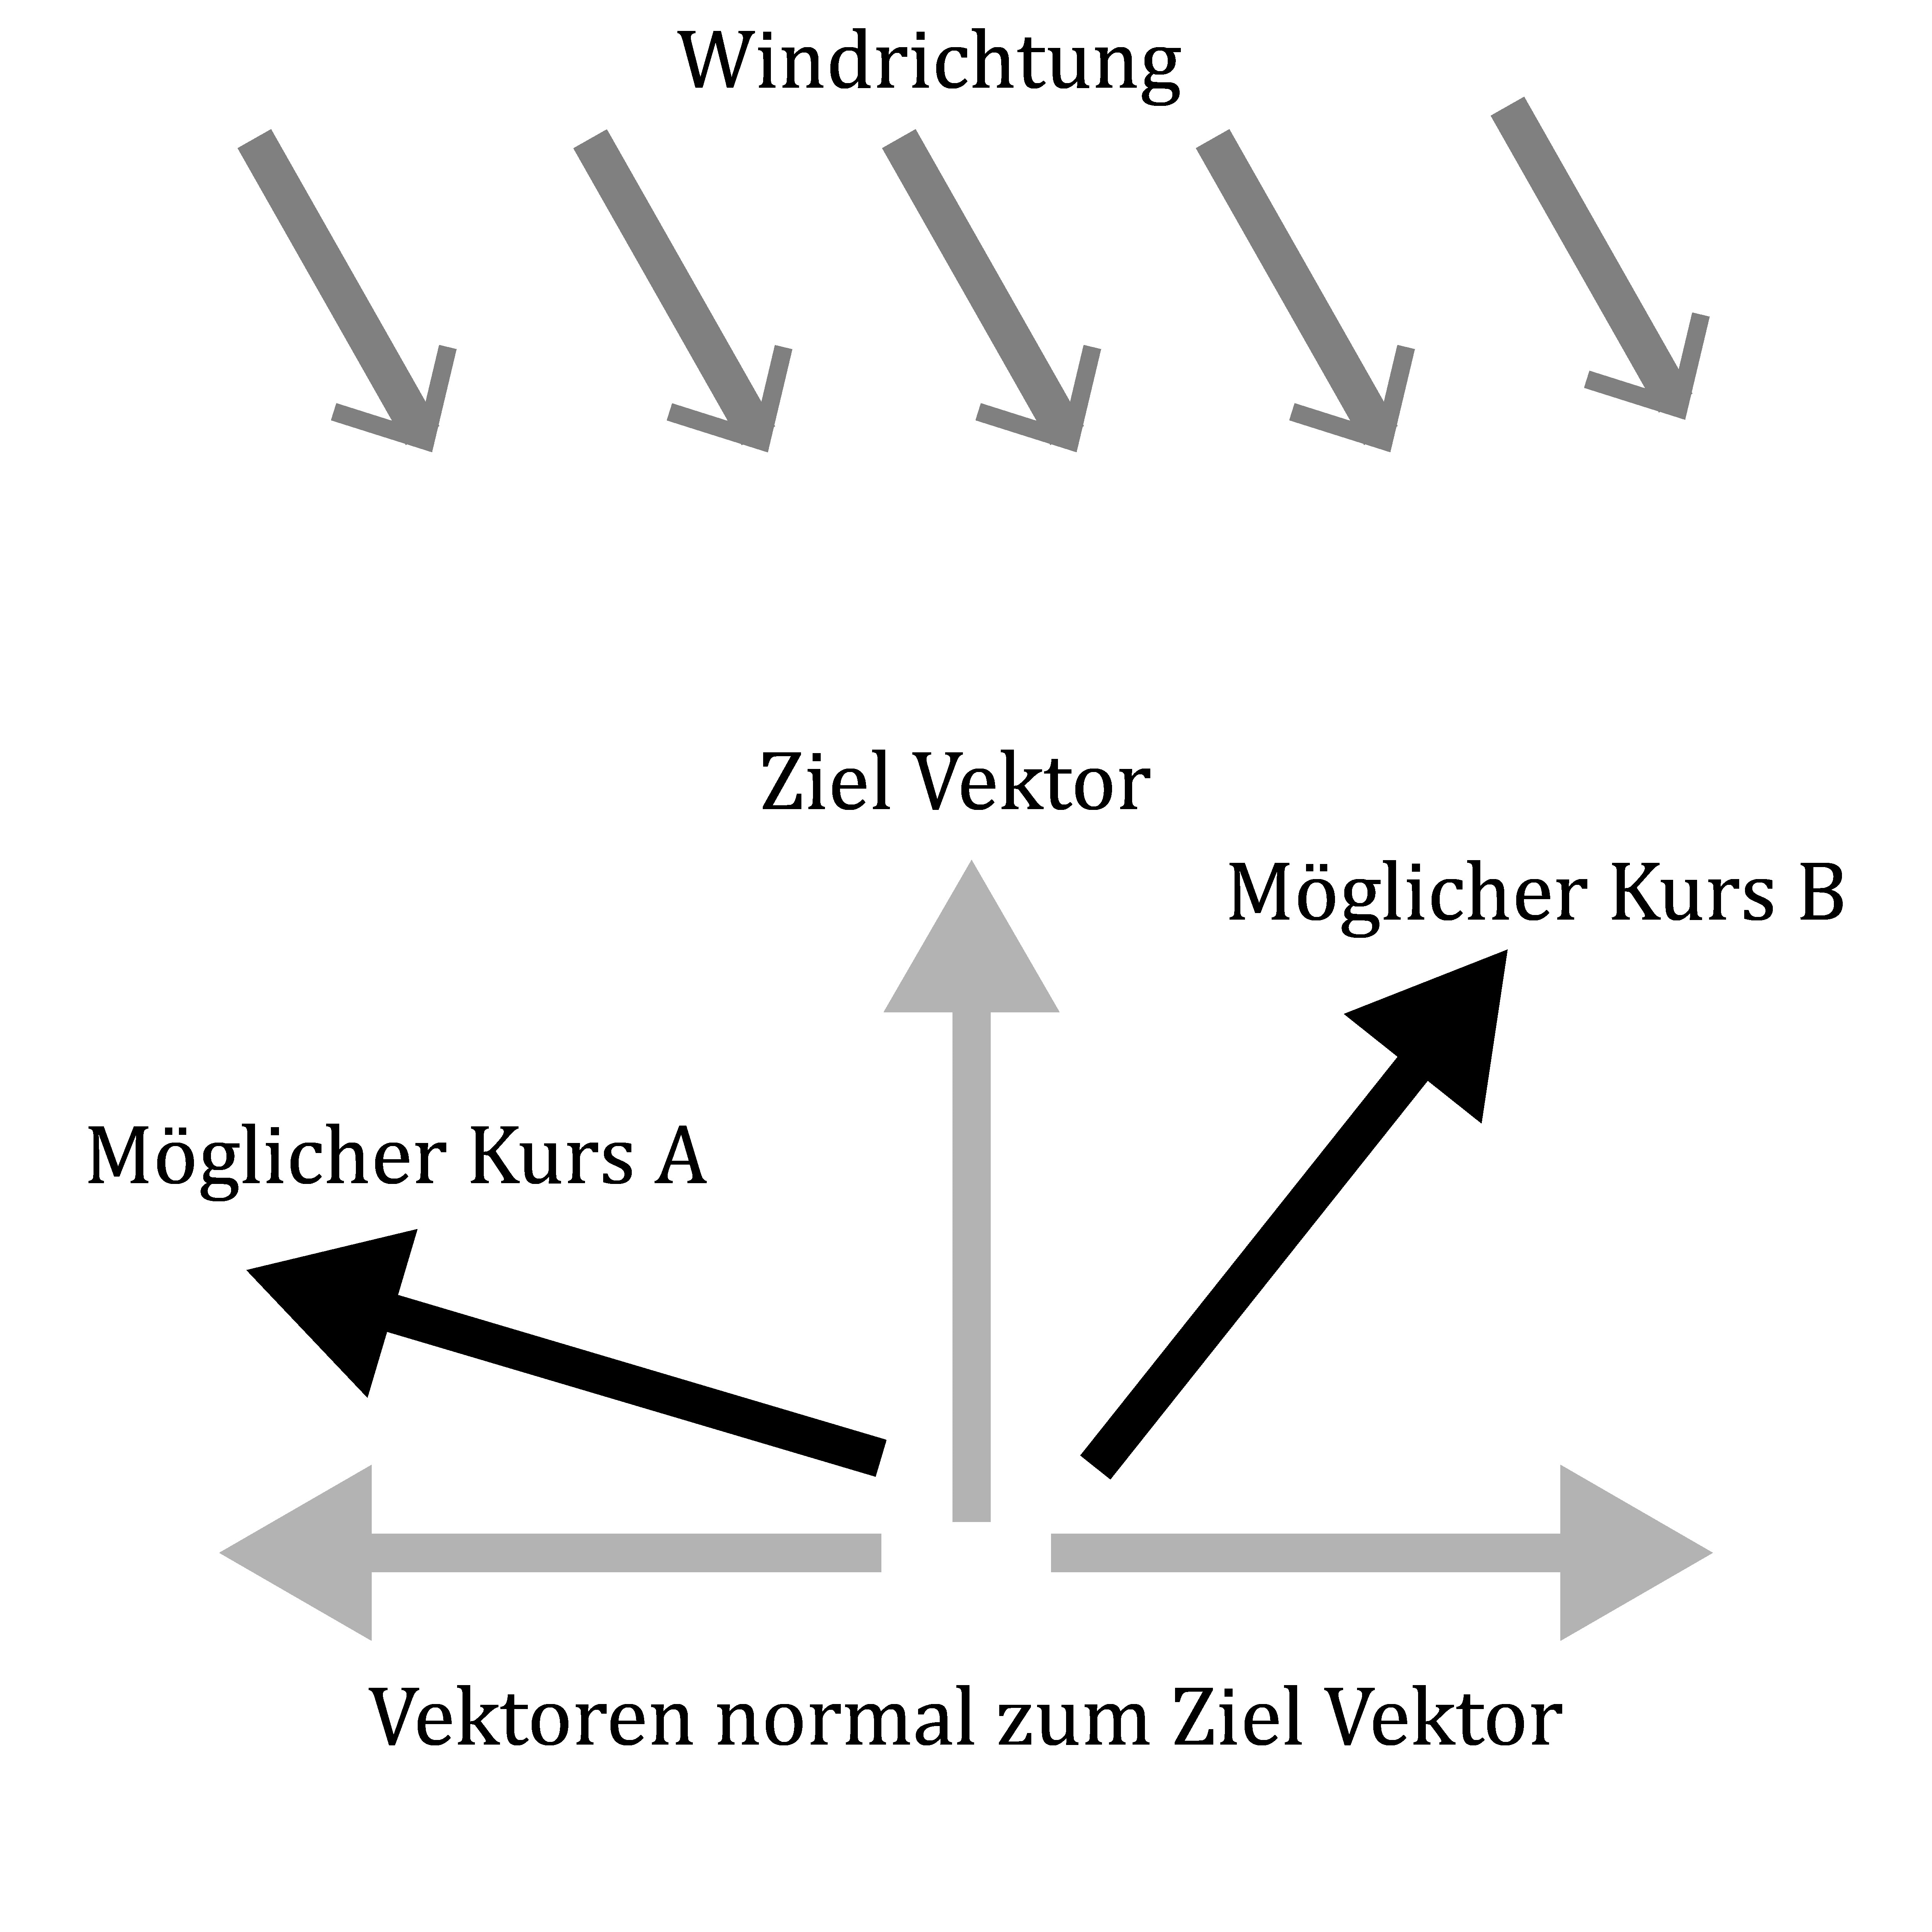
\includegraphics[width=0.5\linewidth]{algorythmus Vektoren.png}
    \caption{Visualisierung der beiden möglichen Pfade}
    \label{fig:enter-label}
\end{figure}
Nun wird wieder mithilfe des Skalarprodukts überprüft, welcher der beiden Kurs-Vektoren näher am Ziel-Vektor ist der dann als nächsten Kurs bestimmt. Der Algorithmus ist ebenfalls im \cref{appendix:algorythmus} nochmals als ganzes zu finden.
\begin{figure}[H]
    \centering
    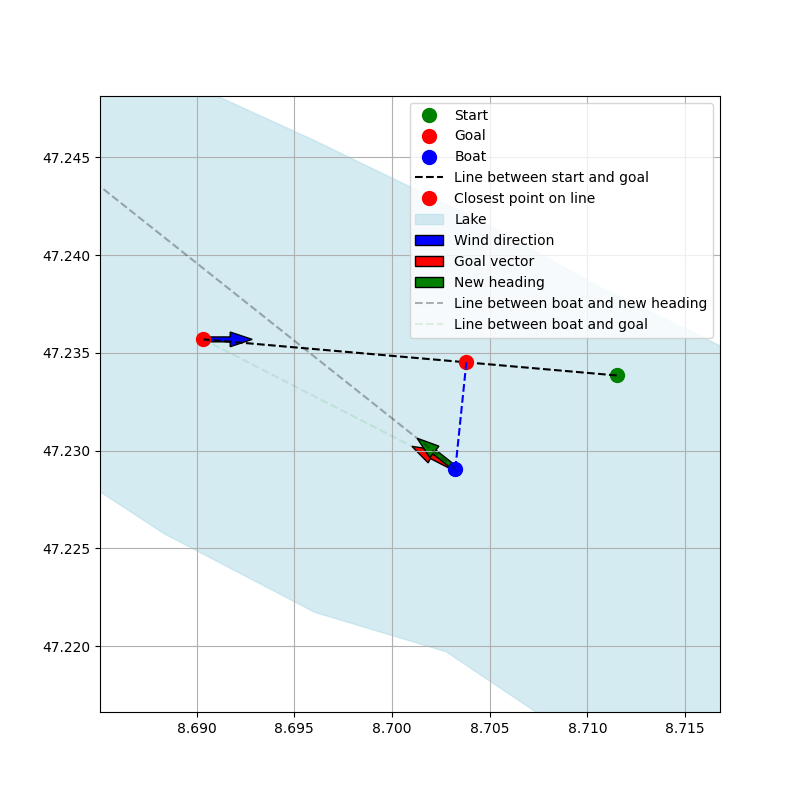
\includegraphics[width=1\linewidth]{assets/3.png}
    \caption{Matplotlib Visualisierung des Algorithmus}
    
\end{figure}

Die Wegpunkte werden Mittels GeoJson bereitgestellt. GeoJson ist grundsätzlich reines Json. Es steht für JavaScript Object Notation und ermöglicht es Objekte von verschienedenen Programiersprachen in einem einheitlichen Format zu speichern. GeoJson ist ein weit verbreitetes Format für Geodaten, da so die Daten standardisiert gespeichert und gelesen werden können.
Das Ziel und die Wegpunkte werden mit Geojson festgelegt. So können diese in diversen Kartenprogrammen einfach bearbeitet werden.

\section{Motorsteuerung}
Wie im Kapitel Elektronik bereits erwähnt, werden zwei Aktuatoren verwendet. Beide lassens ich nur einen 5V plus zwischen 1ms und 2ms auf eine gewünschte Position setzen. 

\subsection{Ruder}
Für das Ruder wird ein PD (Proportional Derivative) Controller verwendet. Auf den Integralen bestandteil kann verzichtet werden, da es sich bei diesen Bewegungen um keine schnellen Bewegungen handelt. 
Um das Ruder auf die gewünsche Position zu stellen, wird als erstes der "Fehler" bzw. der Unterschied zwischen der Aktuellen Ausrichtung und der Gewünschten Ausrichtung berechnet. 
%%% PD controller weiter erklären

\subsection{Segel}
Da das Segel nicht über besonders viele Trimmmöglichkeiten verfügt und die Schnelligkeit wie anfangs erwähnt kein bedeutender Faktor für diese Arbeit ist, wird das Flap immer in die Richtung des Windes gedreht. Dies sorgt dafür, dass das Segel in eine Segelbare Position gebracht wird 

%%%% VISUALISIERUNG 

 
%%% Bereitstellung der Daten mittels GEOJSON







